% One-pager, version 2 (27 September 2026): Same Storm, Different Boats
% Replaces the March 2026 one-pager (onepager.tex, kept unchanged) with the
% results of the Economics Letters revision (main_v3.tex).
% Every number is the paper's or the Online Appendix's; the figure is built
% by src/14_onepager_v2_figure.py from the same exports as the paper.
% Compile with: tectonic onepager_v2.tex

\documentclass[10pt,a4paper]{article}

\usepackage[top=1.1cm, bottom=0.9cm, left=1.7cm, right=1.7cm]{geometry}
\usepackage{graphicx}
\usepackage[dvipsnames]{xcolor}
\usepackage{enumitem}
\usepackage{titlesec}
\usepackage{multicol}
\usepackage{hyperref}
\usepackage[T1]{fontenc}
\usepackage{helvet}
\usepackage{microtype}
\renewcommand{\familydefault}{\sfdefault}

\definecolor{darkblue}{HTML}{1B3A5C}
\definecolor{orange}{HTML}{E8873A}
\definecolor{teal}{HTML}{2E7D6F}
\definecolor{lightgray}{HTML}{F0F0F0}
\definecolor{medgray}{HTML}{777777}

\titleformat{\section}{\small\bfseries\color{darkblue}}{}{0pt}{}
\titlespacing{\section}{0pt}{3pt}{1pt}
\setlength{\columnsep}{0.6cm}
\pagestyle{empty}
\hypersetup{colorlinks=true, urlcolor=teal, linkcolor=teal}

\begin{document}

% === LOGO BAR ===
\noindent
\begin{minipage}[c]{0.15\textwidth}
  
\includegraphics[height=0.95cm]{../assets/logos/orebro_logo.png}
\end{minipage}\hfill
\begin{minipage}[c]{0.13\textwidth}
  
\includegraphics[height=0.7cm]{../assets/logos/ratio_logo.png}
\end{minipage}\hfill
\begin{minipage}[c]{0.09\textwidth}
  
\includegraphics[height=0.7cm]{../assets/logos/ai_econ_lab_logo.png}
\end{minipage}\hfill
\begin{minipage}[c]{0.20\textwidth}\raggedleft
  
\includegraphics[height=0.45cm]{../assets/logos/wasphs_logo.png}
\end{minipage}\hfill
\begin{minipage}[c]{0.20\textwidth}\raggedleft
  
\includegraphics[height=0.7cm]{../assets/logos/aiscaf_logo.png}
\end{minipage}

\vspace{0.1cm}
\noindent\textcolor{darkblue}{\rule{\textwidth}{1.5pt}}

% === TITLE ===
\vspace{0.1cm}
\begin{center}
  {\large\bfseries\color{darkblue} Same Storm, Different Boats:\\[1pt]
  Generative AI and the Age Gradient Within Firms}\\[4pt]
  {\footnotesize \href{https://www.magnuslodefalk.com}{Magnus Lodefalk}\textsuperscript{a,b} \;\textbullet\;
  Lydia L\"othman\textsuperscript{a} \;\textbullet\;
  Michael Koch\textsuperscript{c,d} \;\textbullet\;
  Erik Engberg\textsuperscript{a,b}}\\[1pt]
  {\scriptsize\color{medgray}
  \textsuperscript{a}\"Orebro University \quad
  \textsuperscript{b}Ratio Institute \quad
  \textsuperscript{c}Aarhus University \quad
  \textsuperscript{d}Kiel Institute for the World Economy}
\end{center}

\vspace{-0.1cm}
\noindent\textcolor{darkblue}{\rule{\textwidth}{0.4pt}}

% === KEY FINDING BOX ===
\vspace{0.05cm}
\noindent
\colorbox{lightgray}{%
  \parbox{\dimexpr\textwidth-2\fboxsep}{%
    \vspace{3pt}\centering\small
    {\bfseries\color{darkblue} Key finding:}
    At Swedish employers most exposed to generative AI, the number of
    \textbf{\textcolor{orange}{22--25-year-olds}} relative to their older colleagues
    fell \textbf{\textcolor{orange}{3.9 per cent}} more from 2023 to 2024--25 than at less
    exposed employers. The shortfall falls on \textbf{\textcolor{orange}{young women}},
    and the relative gain \textbf{\textcolor{teal}{rises with age}}.
    \vspace{3pt}
  }%
}

% === FIGURE ===
\vspace{0.1cm}
\begin{center}
  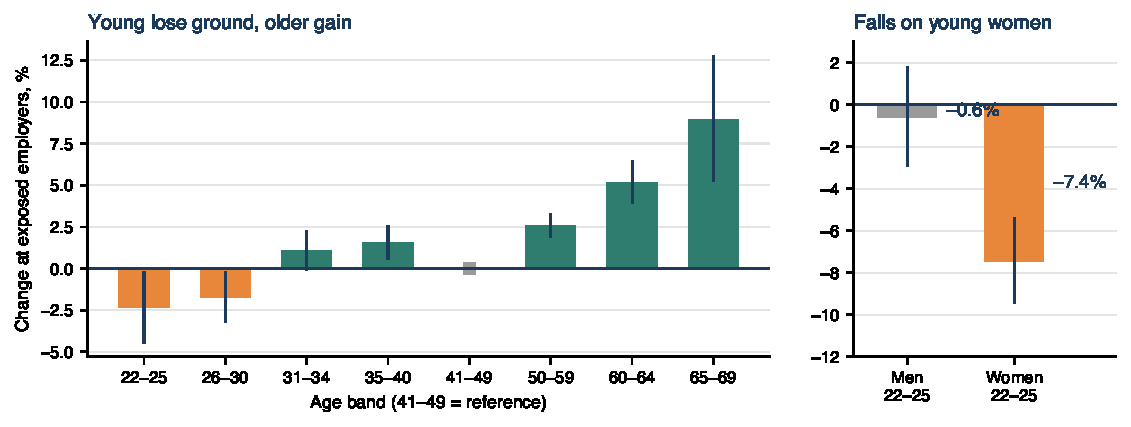
\includegraphics[width=\textwidth]{../figures/onepager_v2_age_sex.pdf}\\[-1pt]
  \parbox{\textwidth}{\scriptsize\color{medgray}
  Change from 2023 to January 2024--June 2025 at the most exposed quarter of employers,
  compared with less exposed employers. Left: each age band against workers aged 41--49
  at the same employers. Right: young women and young men, each against older colleagues
  of the same sex. Lines: 95 per cent confidence intervals.}
\end{center}

% === TWO COLUMNS ===
\vspace{-0.25cm}
\begin{multicols}{2}

\section{What we find}
\begin{itemize}[leftmargin=*, itemsep=1.5pt, parsep=0pt, topsep=0pt]
  \item \textbf{Two shocks, one date apart.} Job postings fell after 2022 while share
        prices rose. The Riksbank's first rate rise came seven months before ChatGPT.
        Which of the two dates the posting decline in exposed occupations follows
        depends on how exposure is measured.
  \item \textbf{Employers shift their advertising.} Within the same employer,
        advertisements for exposed occupations fall about 15 per cent relative to its
        other advertisements after ChatGPT.
  \item \textbf{The young lose ground inside exposed employers.} The young-to-older
        employment ratio falls 3.9 per cent more at ages 22--25 and at ages 26--30. The
        relative gain rises with age, to 8.9 per cent at 65--69 against 41--49.
  \item \textbf{Young women bear the shortfall.} Young women lose 7.4 per cent against
        their older colleagues; young men do not change. The gap is measured inside the
        same employers and survives largely within fields of education.
  \item \textbf{Separations rise, hires do not fall.} Relative separations of the
        young rise, though imprecisely once industries may differ. More than half of employees under 25
        hold fixed-term contracts, so a contract not renewed counts as a separation.
\end{itemize}

\section{How much weight it bears}
\begin{itemize}[leftmargin=*, itemsep=1.5pt, parsep=0pt, topsep=0pt]
  \item The result describes \textbf{who works at exposed employers}, not how many
        jobs exist in the economy.
  \item It largely holds against industry-wide movements, firm debt (the credit channel of
        tightening), remote work and pension-age changes. On an alternative exposure
        measure the women's result is unchanged and the pooled estimate less precise.
  \item The ratio also moved in the pandemic year, but then it fell on young men.
\end{itemize}

\section{Why it matters for policy}
\begin{itemize}[leftmargin=*, itemsep=1.5pt, parsep=0pt, topsep=0pt]
  \item \textbf{Watch composition, not only totals.} A reshuffling inside employers is
        invisible in aggregate employment and posting counts.
  \item \textbf{Entry routes matter.} Fixed-term first jobs are where the adjustment
        shows; work-integrated learning and vocational routes (YH) that build experience
        with AI tools deserve attention, for young women in particular.
  \item \textbf{Timely occupational statistics.} Occupation codes arrive about two years
        late, and on their own they can manufacture a spurious youth decline.
\end{itemize}

\end{multicols}

% === FOOTER ===
\vspace{-0.15cm}
\noindent\textcolor{darkblue}{\rule{\textwidth}{0.4pt}}
\vspace{0.02cm}

\noindent
{\scriptsize\color{medgray}
\textbf{Data and method:} Monthly employer declarations (arbetsgivardeklarationer p\aa{}
individniv\aa{}) from Statistics Sweden, covering every employee in Sweden, January 2021 to
June 2025, and 4.9 million Platsbanken job advertisements. An employer's exposure is fixed
from the 2019 occupations of its workers aged 31--69, scored with the DAIOE index
(Engberg et al.), so no young worker's current occupation is needed. Poisson estimates
comparing age groups within 104{,}217 employers, with employer-by-month and age-by-month
effects; standard errors clustered by employer.
\hfill \textbf{27 September 2026}\\[1pt]
\textit{Revised working paper,} \href{https://www.ai-econlab.com/papers}{ai-econlab.com/papers}
\;\textbullet\; Code: \href{https://github.com/Magnus-L/canaries-sweden}{github.com/Magnus-L/canaries-sweden}
\;\textbullet\; Part of \href{https://www.aiscaf.se}{AISCAF} (\href{https://wasp-hs.org}{WASP-HS})
and the \href{https://www.ai-econlab.com}{AI-Econ Lab}}

\vspace{0.03cm}
\noindent
{\scriptsize\color{medgray}
\textbf{Contact:}
Lydia L\"othman, \href{mailto:lydia.lothman@oru.se}{lydia.lothman@oru.se}, 070-9584726
\;\textbullet\;
Magnus Lodefalk, \href{mailto:magnus.lodefalk@oru.se}{magnus.lodefalk@oru.se}, 0722-217340}

\end{document}
